\begin{center}
    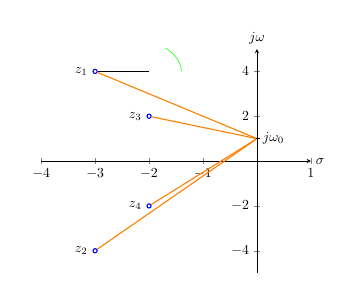
\begin{tikzpicture}
        [
            scale = 0.5,
            >=latex,
            ns/.style={circle, draw=blue, fill=white, thick, inner sep=0pt, minimum size=3pt}
            %pol/.style={cross, draw=blue, thick} not working with crosses
        ]
        \begin{axis}
            [
                xmin=-4, xmax=1, ymin=-5, ymax=5, axis lines=middle,
                x label style={anchor=west},
                xlabel=$\sigma$,
                y label style={anchor=south},
                ylabel=$j \omega$,
                %grid
            ]
            
            % nodes
            \node[label=right: $j \omega_0$, inner sep = 0pt]        (freq0)     at (0, 1)       {};
            \node[ns, label=left: $z_1$]            (z1)        at (-3, 4)      {};
            \node[ns, label=left: $z_2$]            (z2)        at (-3, -4)     {};
            \node[ns, label=left: $z_3$]            (z3)        at (-2, 2)      {};
            \node[ns, label=left: $z_4$]            (z4)        at (-2, -2)     {};
            
            \draw                       (-0.05, 1) -- (0.05, 1);
            \draw[thick, orange]        (freq0) to (z1);
            \draw[thick, orange]        (freq0) to (z2);
            \draw[thick, orange]        (freq0) to (z3);
            \draw[thick, orange]        (freq0) to (z4);
            \draw                       (z1) -- (-2, 4);
            % \draw[arc]                  at (-2, 4) +(30:60:1cm);
            \draw[green]                (-1.4, 4) arc (0:150:2);
            
           
        \end{axis}
        
    \end{tikzpicture}
\end{center}